\subsection{Geometry}
\begin{itemize}
   \item latest geometry in Figure \ref{fig:init}
   \item corresponding electric field for $p=3$, $n_\mathrm{sub}=16$,  $V_\mathrm{el}=-300\ \mathrm{kV}$ and $V_\mathrm{ar}=1\ \mathrm{kV}$
   \item (patches $32 \dots 35$ are not correct, missing the correct high voltage adapter)
\end{itemize}

\begin{center}
\begin{figure}[H]
   \begin{subfigure}{0.45\textwidth}
      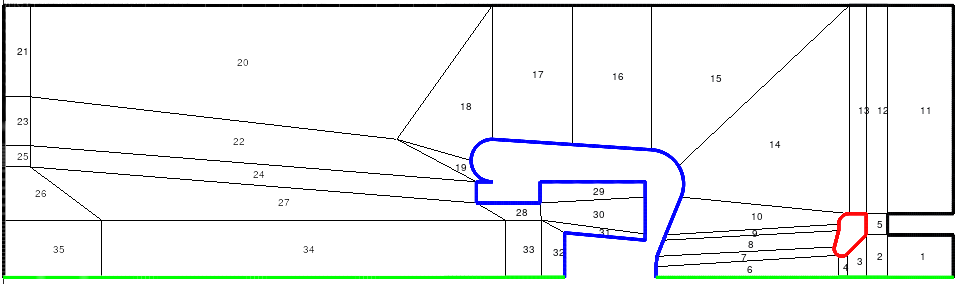
\includegraphics[width=\textwidth]{fig/geometry_v6}
      % \caption{geometry}
      % \label{fig:geometry_v6}
   \end{subfigure}
   \begin{subfigure}{0.45\textwidth}
      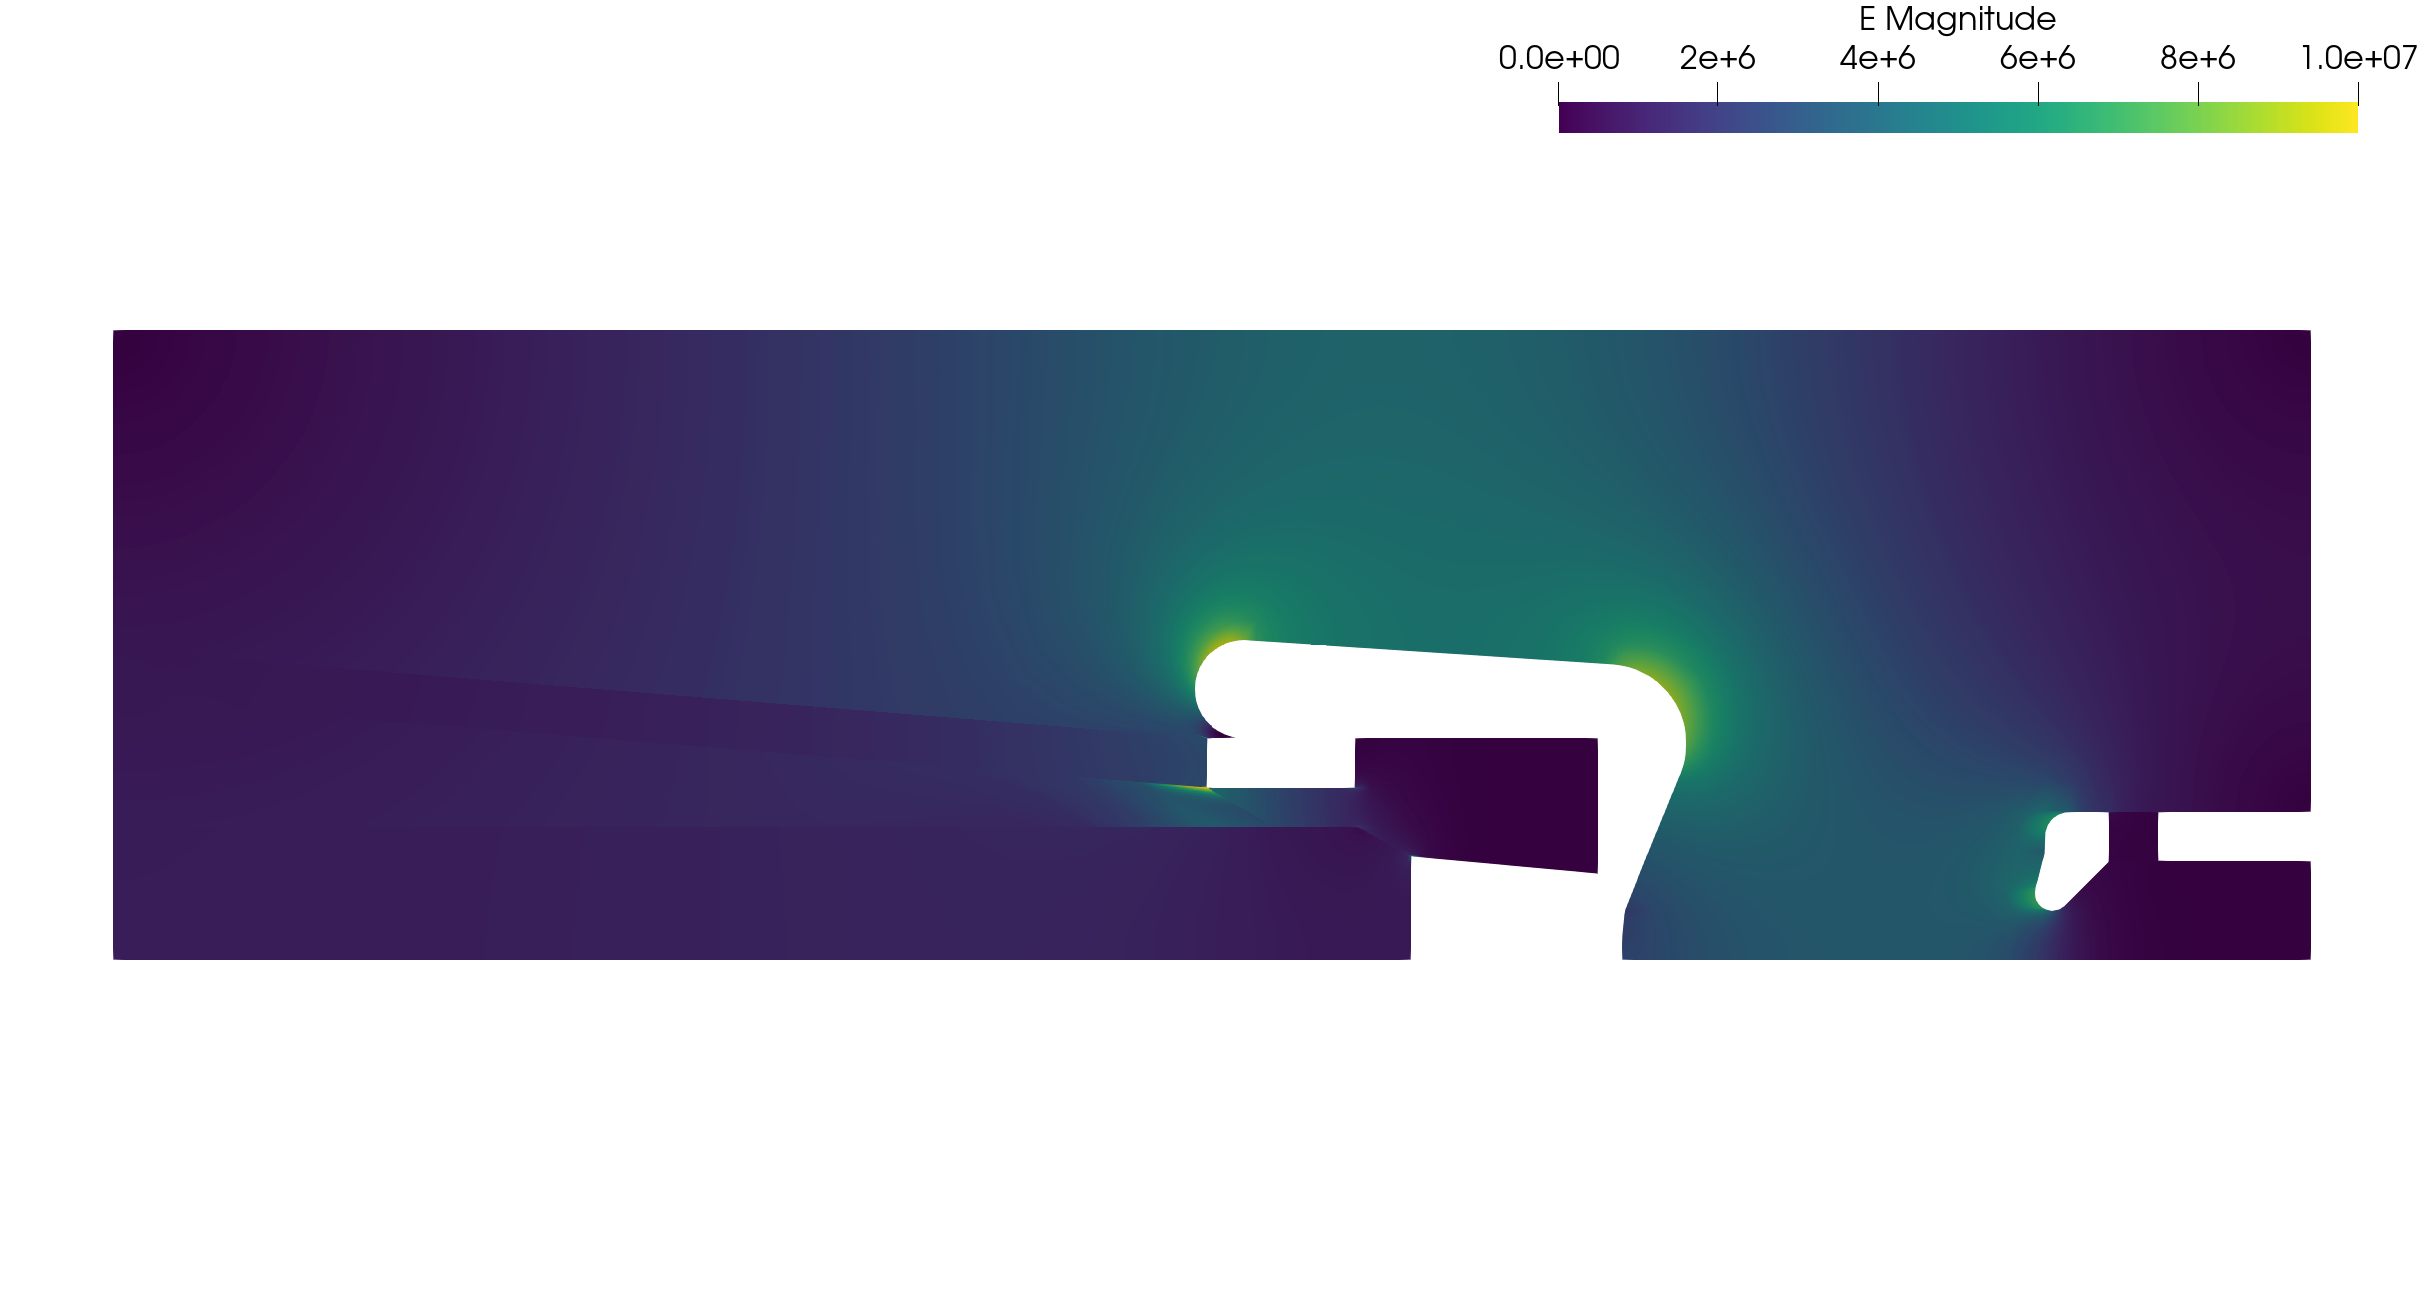
\includegraphics[width=\textwidth]{fig/E_v6}
      % \caption{magnitude of electric field}
      % \label{fig:E_v6}
   \end{subfigure}
   \caption{initial geometry and electric field}
   \label{fig:init}
\end{figure}
\end{center}

\subsection{Optimization}
\begin{itemize}
   \item optimized geometry in Figure \ref{fig:opt}
   \item cost function only takes into account electric field
   \item only the upper electrode shape is optimized (volume constrained could be kept as before at $625\ \mathrm{cm}^3$)
   \item corresponding electric field for $p=3$, $n_\mathrm{sub}=16$,  $V_\mathrm{el}=-300\ \mathrm{kV}$ and $V_\mathrm{ar}=1\ \mathrm{kV}$
   \item \textbf{magnitude of E-field remains large in patch 14}
\end{itemize}

\begin{center}
\begin{figure}[H]
   \begin{subfigure}{0.45\textwidth}
      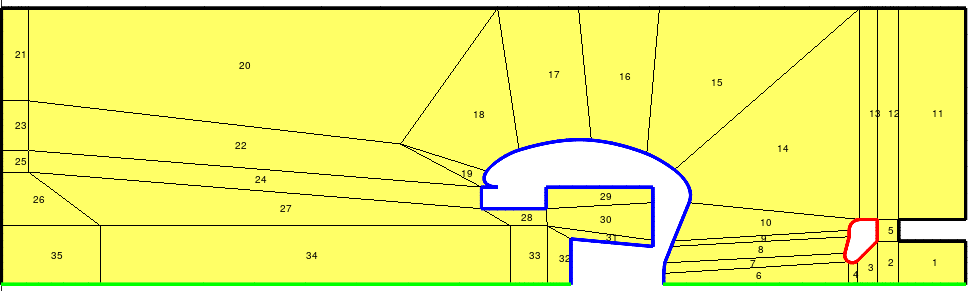
\includegraphics[width=\textwidth]{fig/geometry_v6_opt_order=3_run1}
      % \caption{geometry}
      % \label{fig:geometry_v6_opt}
   \end{subfigure}
   \begin{subfigure}{0.45\textwidth}
      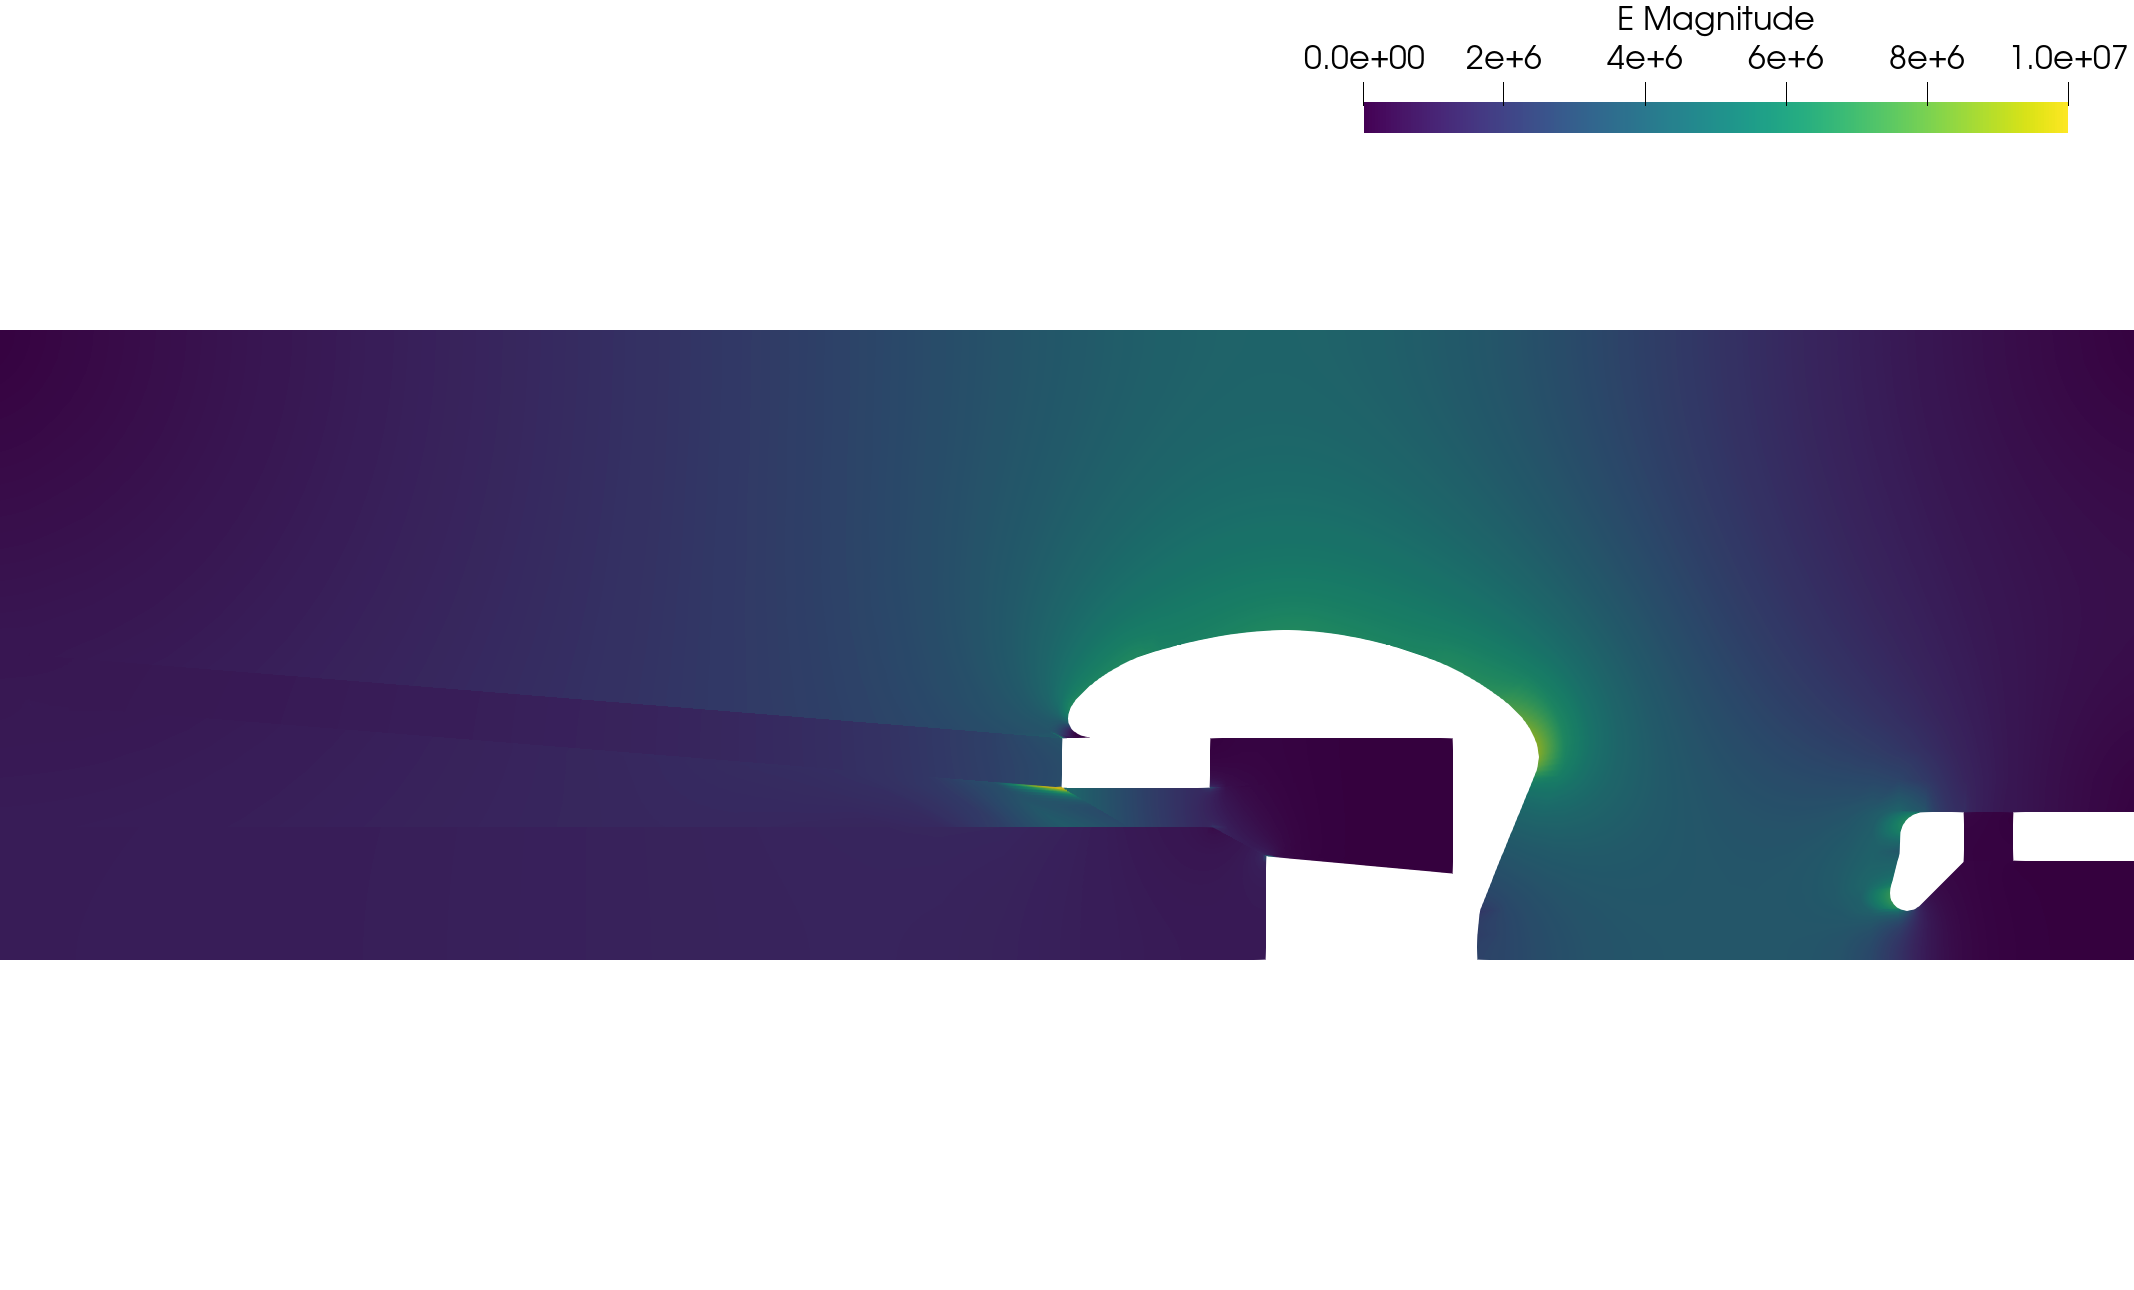
\includegraphics[width=\textwidth]{fig/E_v6_opt_order=3_run1}
      % \caption{magnitude of electric field}
      % \label{fig:E_v6_opt}
   \end{subfigure}
   \caption{optimized geometry and electric field}
   \label{fig:opt}
\end{figure}
\end{center}

\subsection{Tracking}
\begin{itemize}
   \item \textbf{general settings}: $Q=100\ \mathrm{fC}$, $\tau_\mathrm{b}=30\ \mathrm{ps}$
   \item \textbf{initial distribution}: Gaussian with $\sigma=400\ \mu\mathrm{m}$, see Figure \ref{fig:generator} for comparison with laser measurement (probe particles at $0.5\sigma$, $\sigma$, $1.5\sigma$ in red)
\end{itemize}

\begin{center}
\begin{figure}[H]
   \begin{subfigure}{0.45\textwidth}
      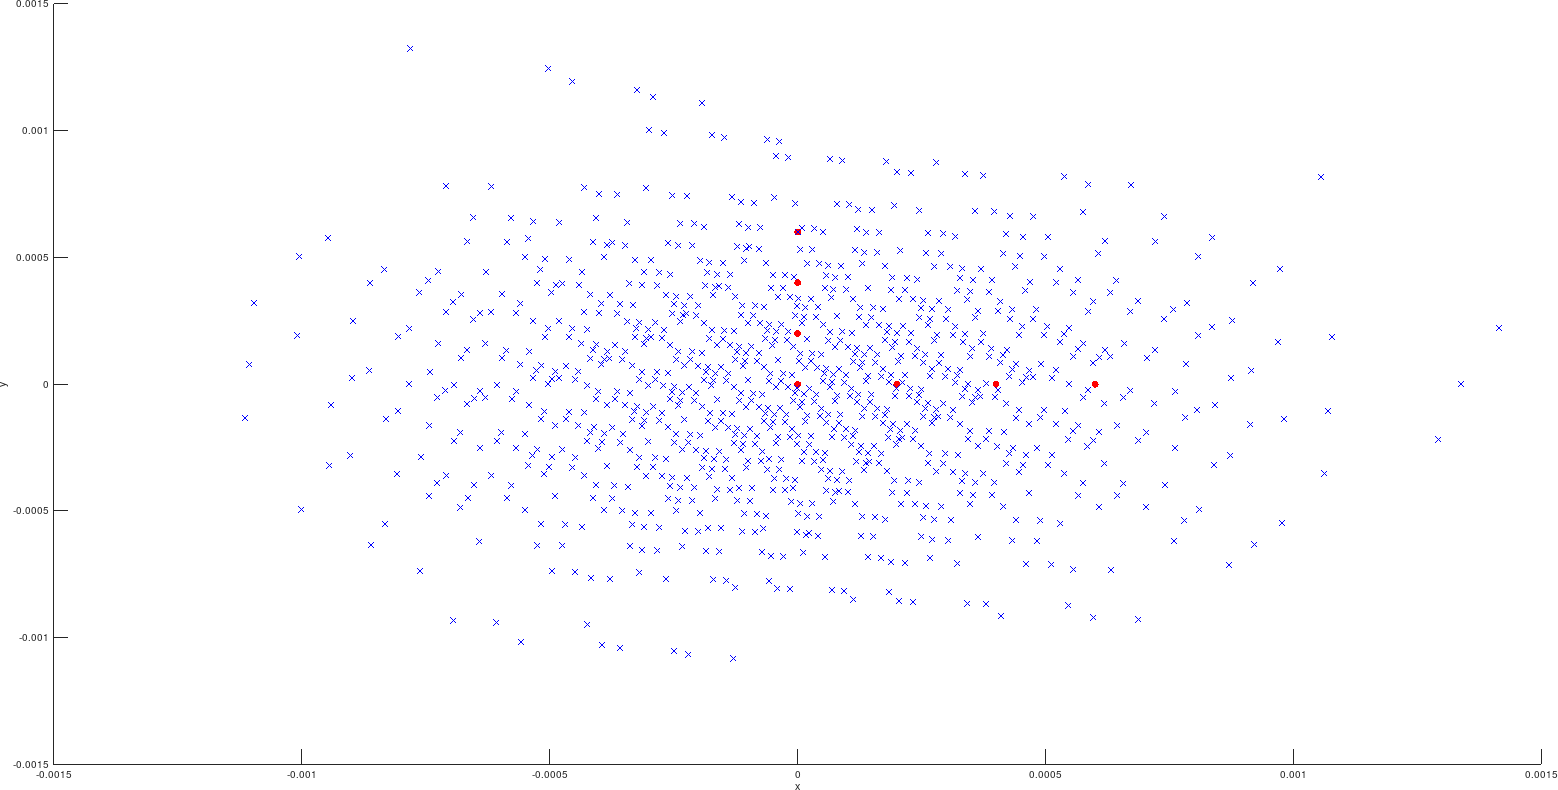
\includegraphics[width=\textwidth]{fig/generator}
   \end{subfigure}
   \begin{subfigure}{0.45\textwidth}
      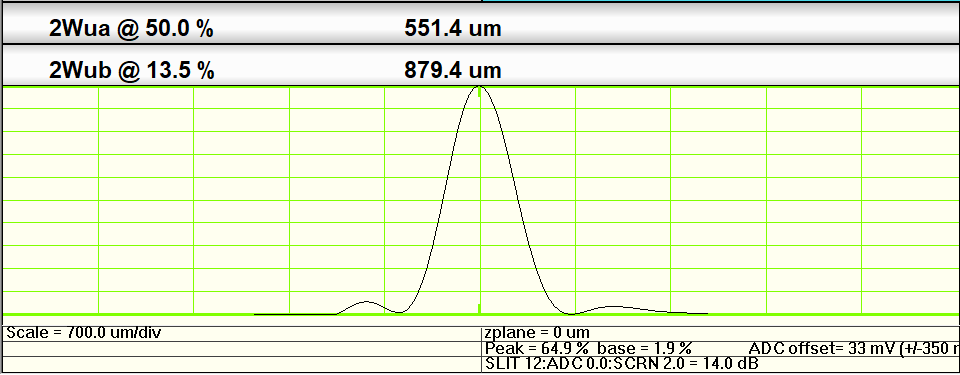
\includegraphics[width=\textwidth]{fig/laser}
   \end{subfigure}
   \caption{initial distribution (1000 particles) and laser measurement}
   \label{fig:generator}
\end{figure}
\end{center}

\begin{itemize}
   \item \textbf{convergence of time integrator}: error of normalized transversal emmitance $\epsilon$ is shown in Figure \ref{fig:int_cvg} ($H=2^{-11}\ \mathrm{ns}$ used later on)\\
\end{itemize}

\begin{center}
\begin{figure}[H]
   \begin{subfigure}{0.45\textwidth}
      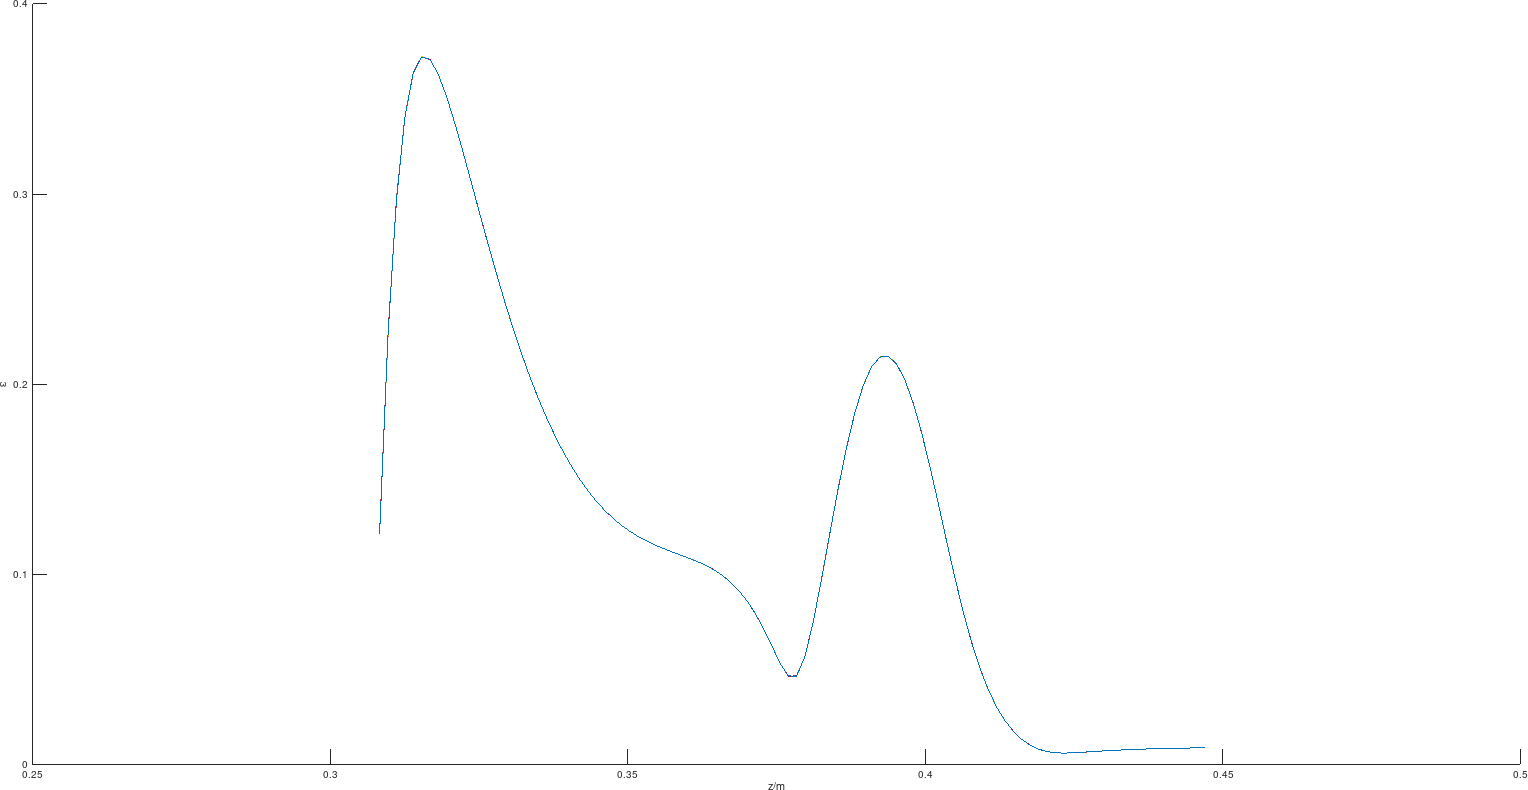
\includegraphics[width=\textwidth]{fig/int_emit}
   \end{subfigure}
   \begin{subfigure}{0.45\textwidth}
      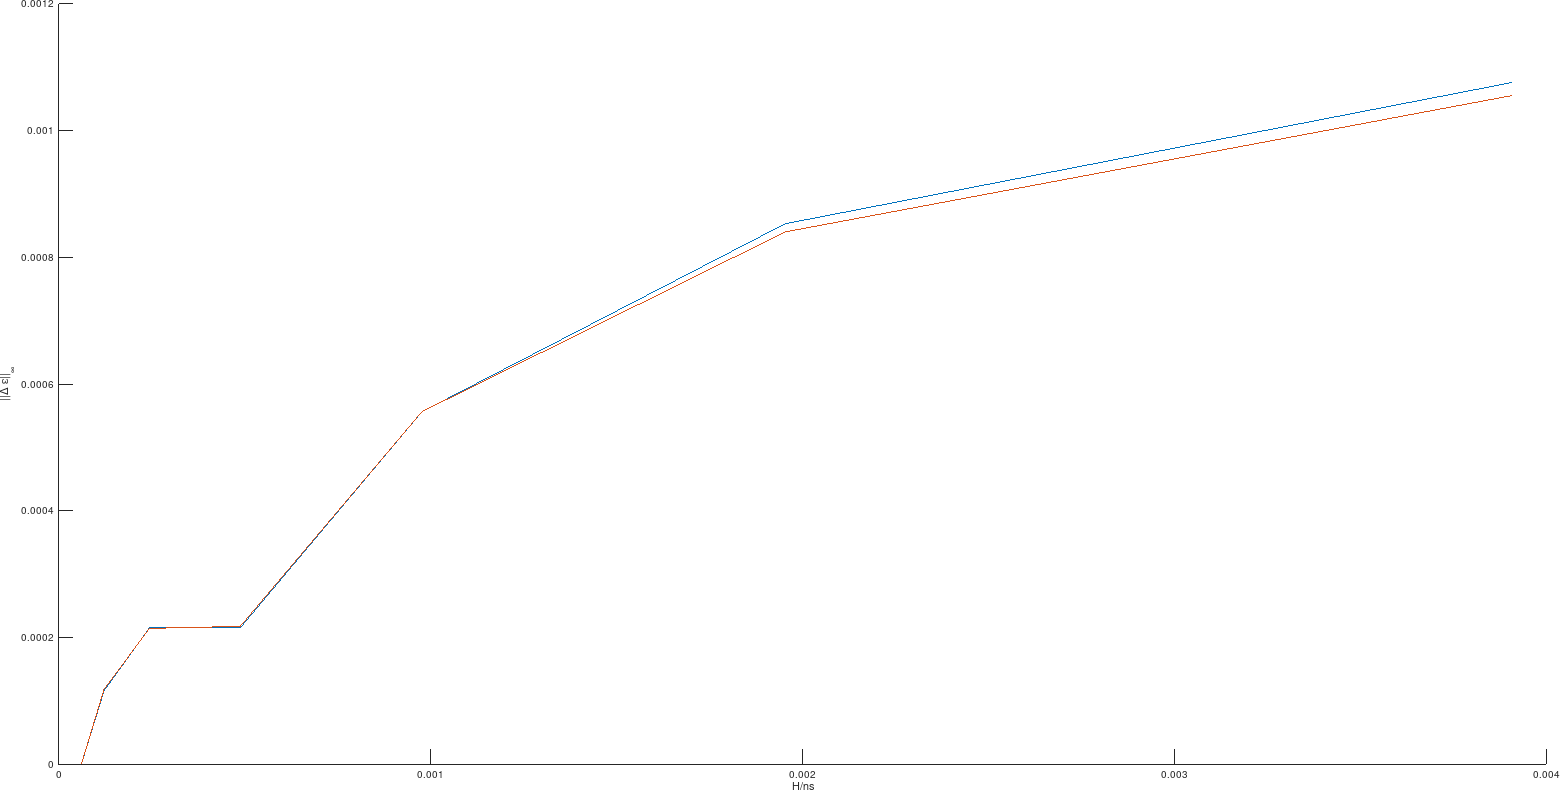
\includegraphics[width=\textwidth]{fig/int_cvg}
   \end{subfigure}
   \caption{normalized transversal emmitance and absolute error of time integrator in $l_\infty$-norm}
   \label{fig:int_cvg}
\end{figure}
\end{center}

\begin{itemize}
   \item \textbf{convergence of field map}: look at convergence in transversal $n_x, n_y$ and longitudinal $n_z$ direction with number of interpolation points given by $2^n$
   \item Figure \ref{fig:map_cvg_xy} looks at convergence of $n_x, n_y$ for $n_z$ large and fixed
   \item Figure \ref{fig:map_cvg_z} looks at convergence of $n_z$ for $n_x=n_y=4$ fixed
   \item $n_x=n_y=4$ and $n_z=6$ used later on
\end{itemize}

\begin{center}
\begin{figure}[H]
   \begin{subfigure}{0.45\textwidth}
      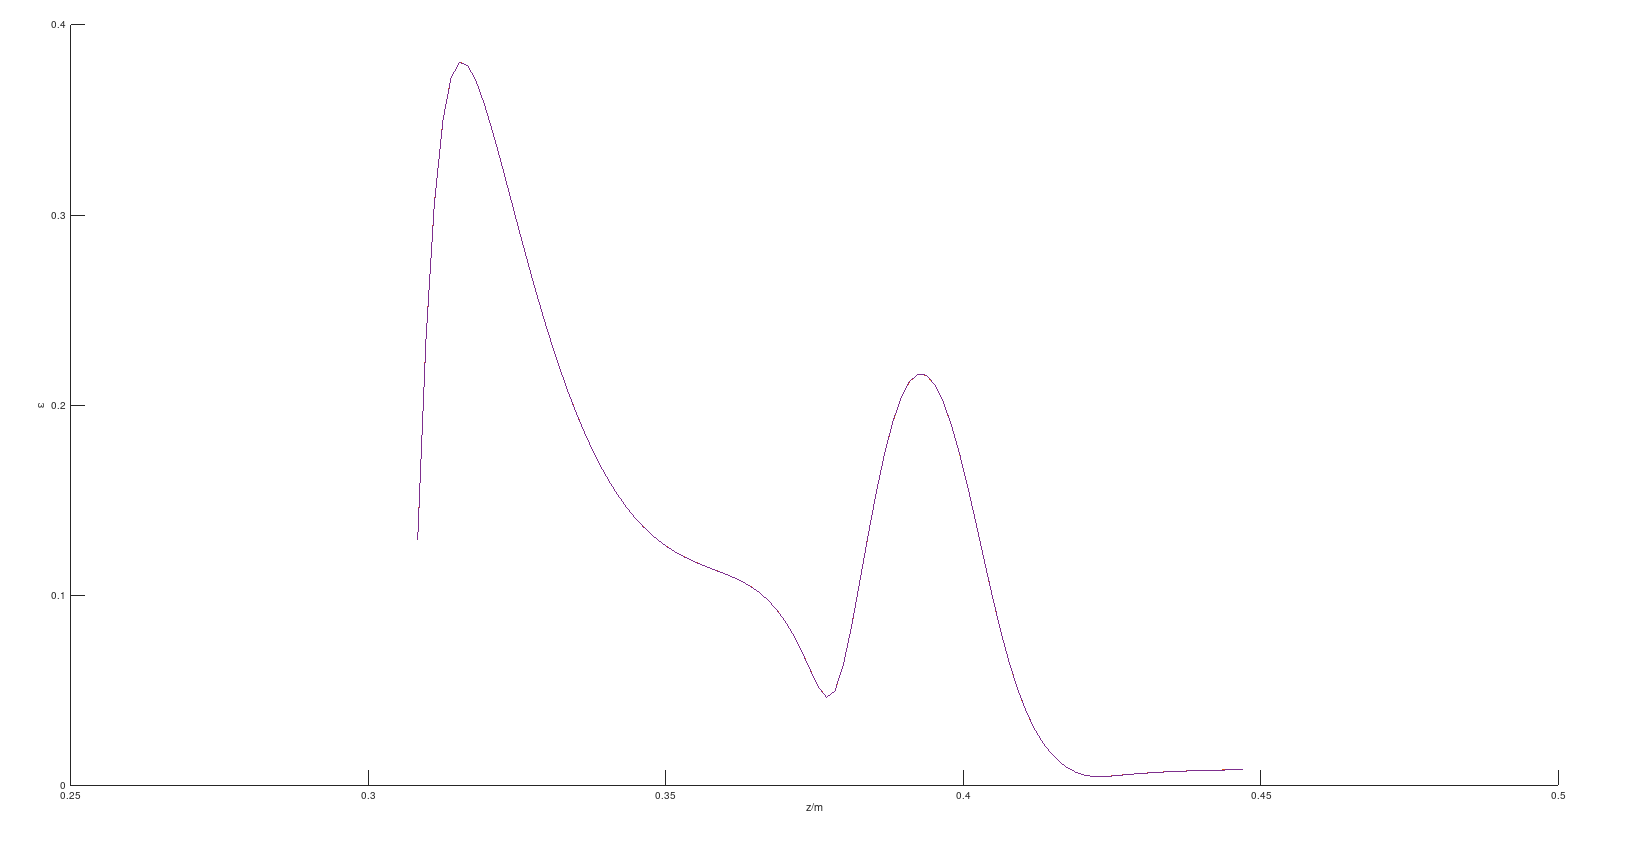
\includegraphics[width=\textwidth]{fig/map_emit_xy}
   \end{subfigure}
   \begin{subfigure}{0.45\textwidth}
      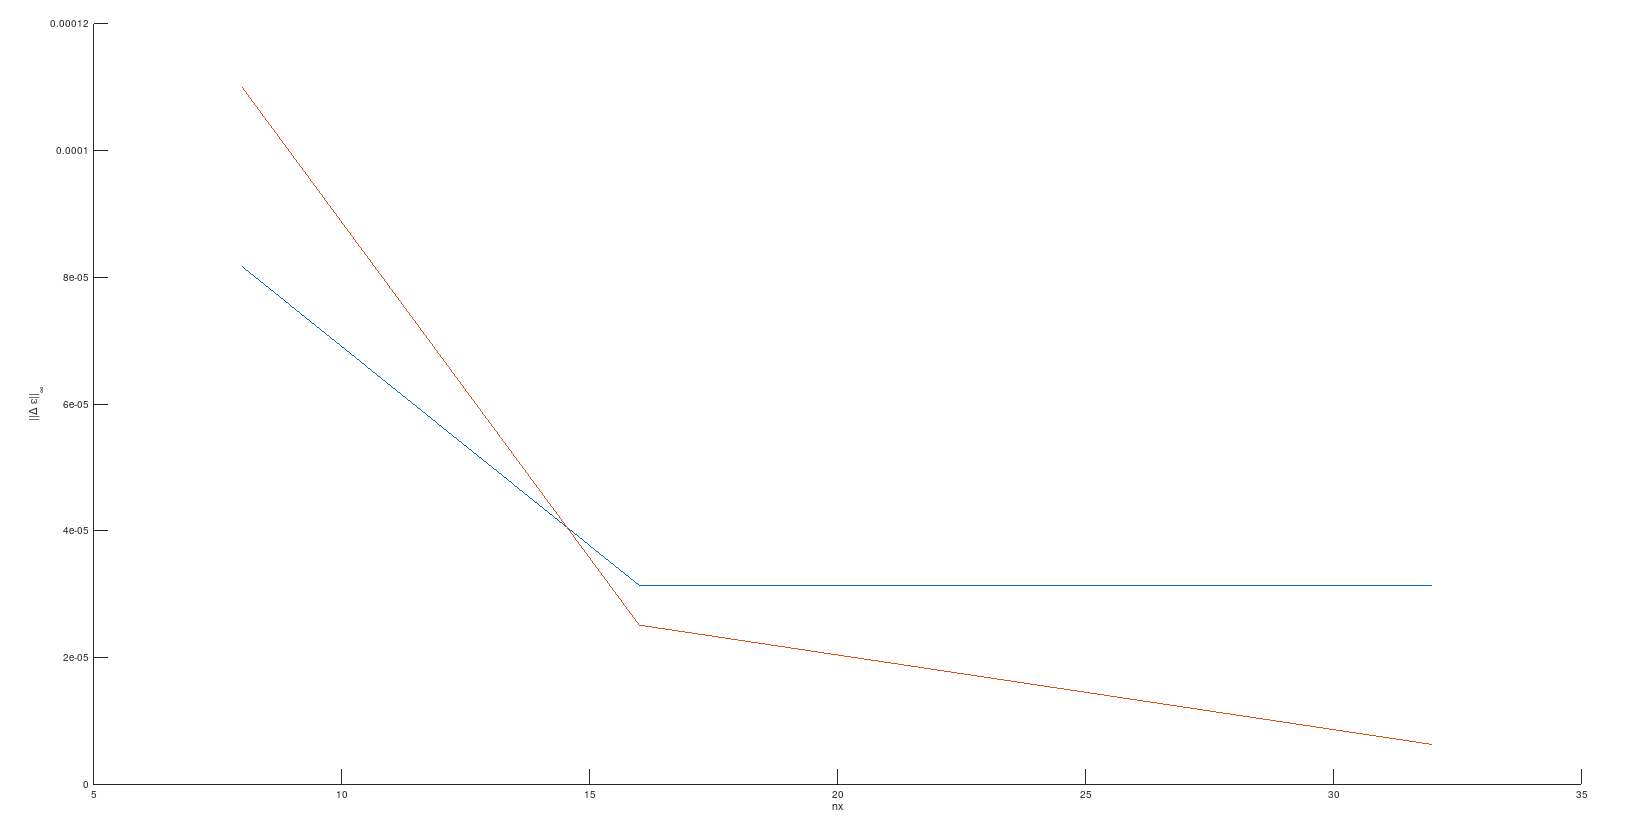
\includegraphics[width=\textwidth]{fig/map_cvg_xy}
   \end{subfigure}
   \caption{normalized transversal emmitance and absolute error of field map in $l_\infty$-norm for $n_z=6$ and $n_x=n_y$ variable}
   \label{fig:map_cvg_xy}
\end{figure}
\end{center}

\begin{center}
\begin{figure}[H]
   \begin{subfigure}{0.45\textwidth}
      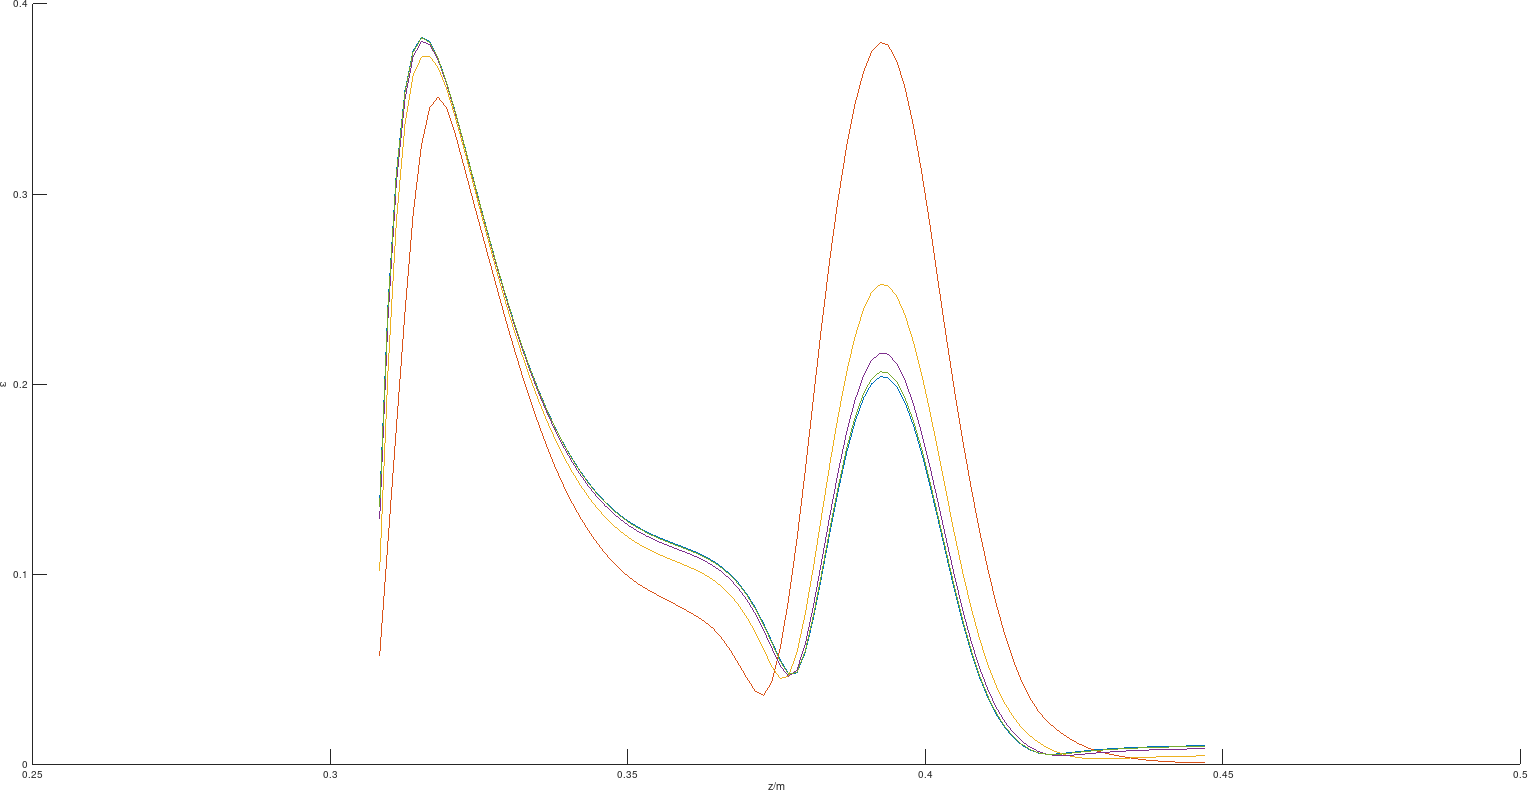
\includegraphics[width=\textwidth]{fig/map_emit_z}
   \end{subfigure}
   \begin{subfigure}{0.45\textwidth}
      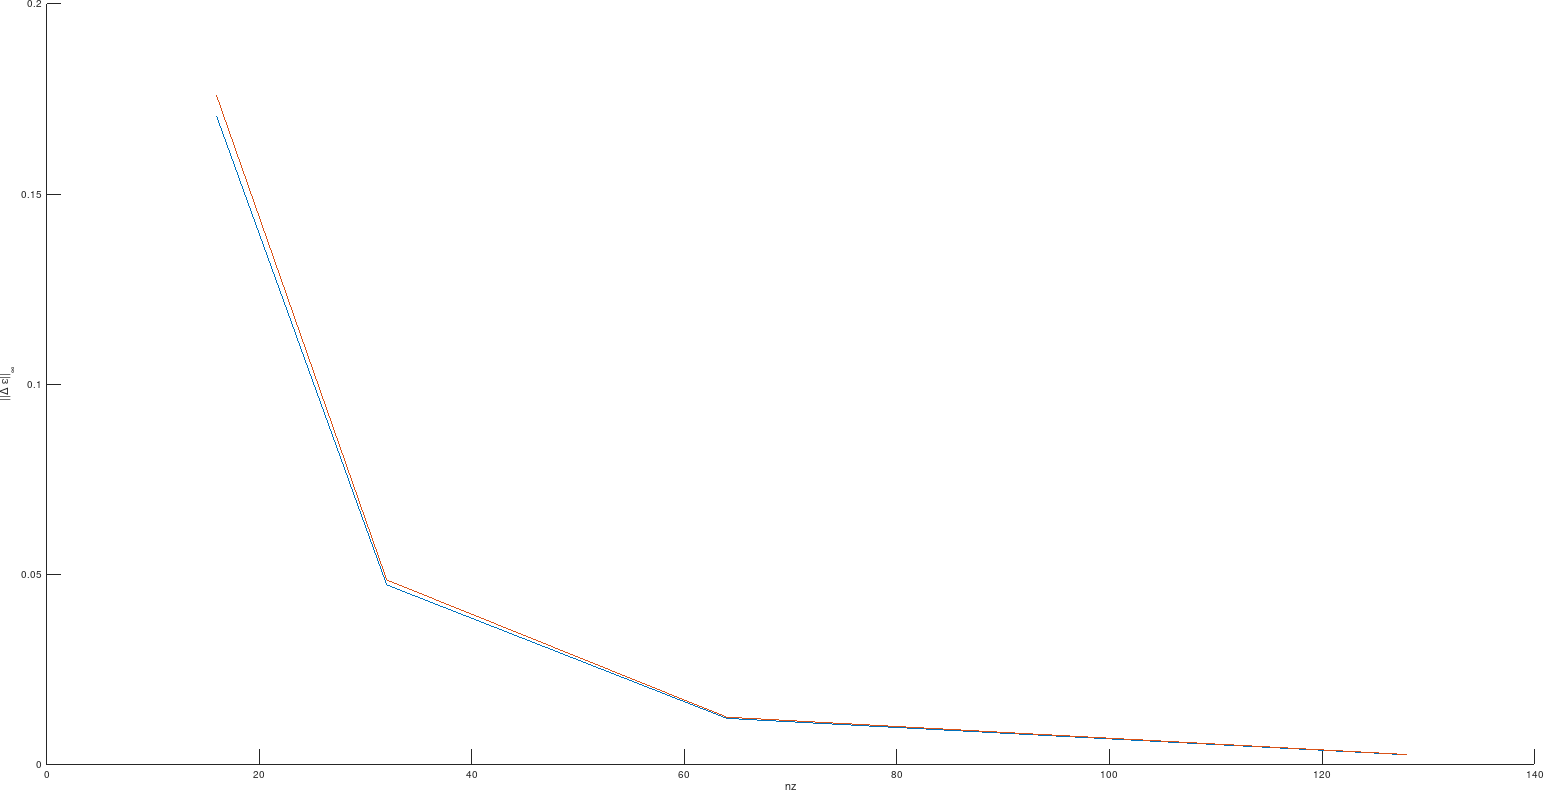
\includegraphics[width=\textwidth]{fig/map_cvg_z}
   \end{subfigure}
   \caption{normalized transversal emmitance and absolute error of field map in $l_\infty$-norm for $n_z$ variable and $n_x=n_y=4$}
   \label{fig:map_cvg_z}
\end{figure}
\end{center}

\begin{itemize}
   \item \textbf{convergence of space charge}: look at convergence of grid $n_r, n_l$ and number of particles $n_I$ separately with number of grid cells or particles given by $2^n$

   \item Figure \ref{fig:sc_cvg_rl} looks at convergence of $n_r, n_l$ for $n_I=10$ large and fixed
   \item $n_r$ seems to have a more profound impact, but neither seem to affect the solution too much for $n\geq8$

   \item Figure \ref{fig:sc_cvg_I} looks at convergence of $n_I$ for $n_r=n_l=4$
   \item $n_r=n_l=4$ and $n_I=10$ seem sufficient
\end{itemize}

\begin{center}
\begin{figure}[H]
   \begin{subfigure}{0.45\textwidth}
      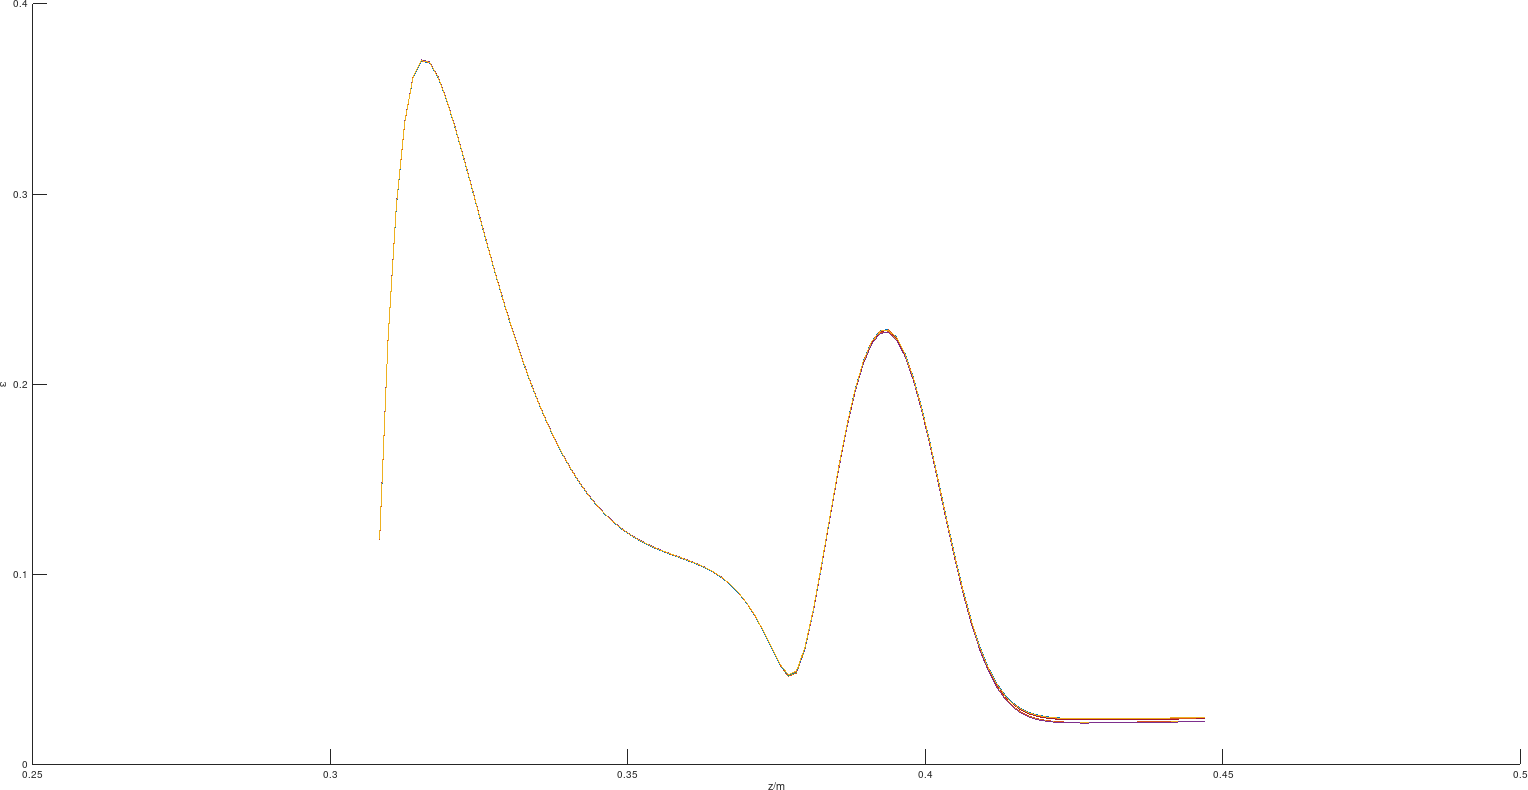
\includegraphics[width=\textwidth]{fig/sc_emit_rl}
   \end{subfigure}
   \begin{subfigure}{0.45\textwidth}
      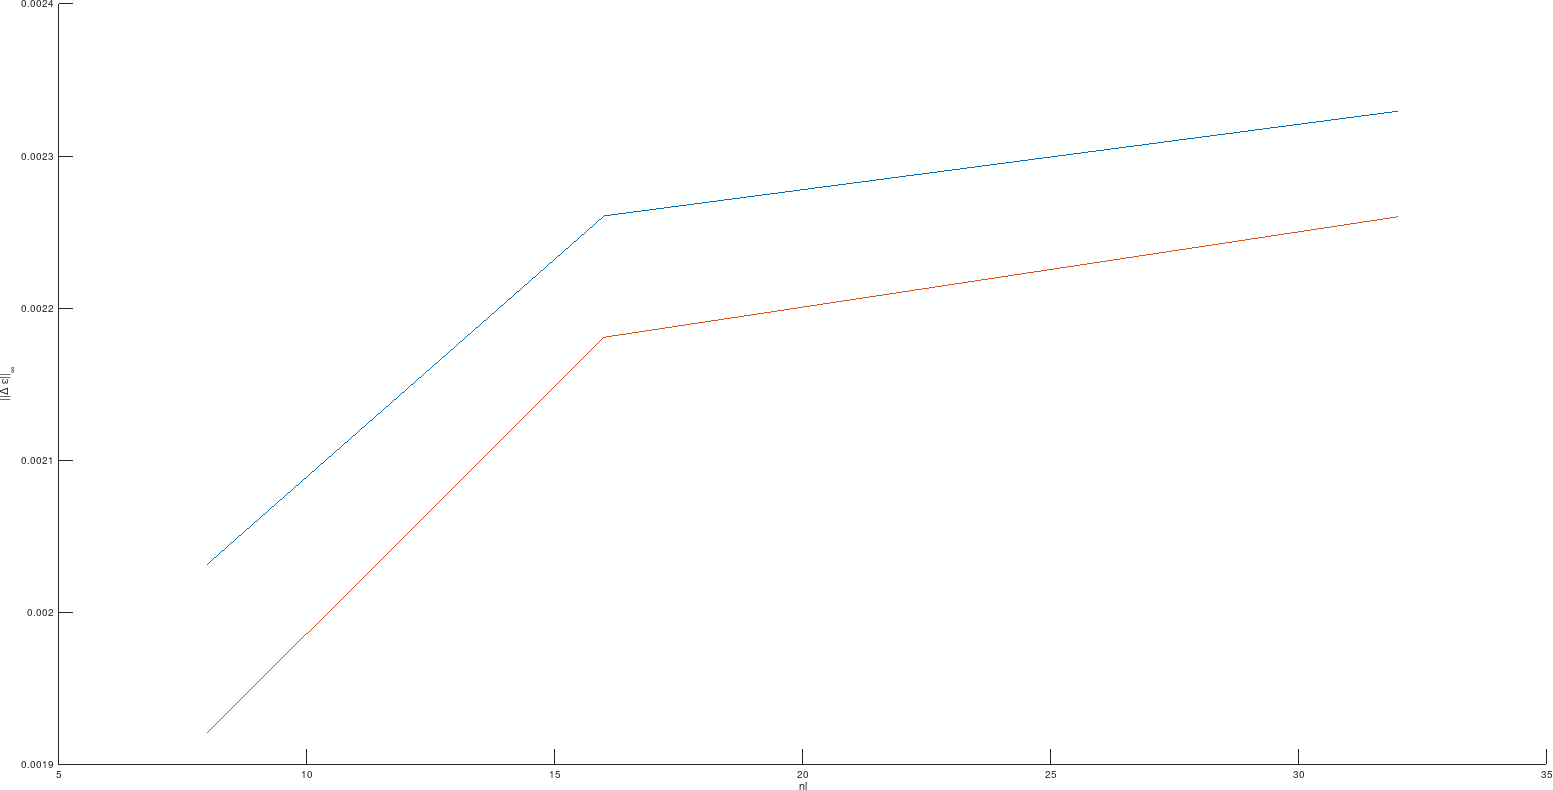
\includegraphics[width=\textwidth]{fig/sc_cvg_rl=3}
   \end{subfigure}

   \begin{subfigure}{0.45\textwidth}
      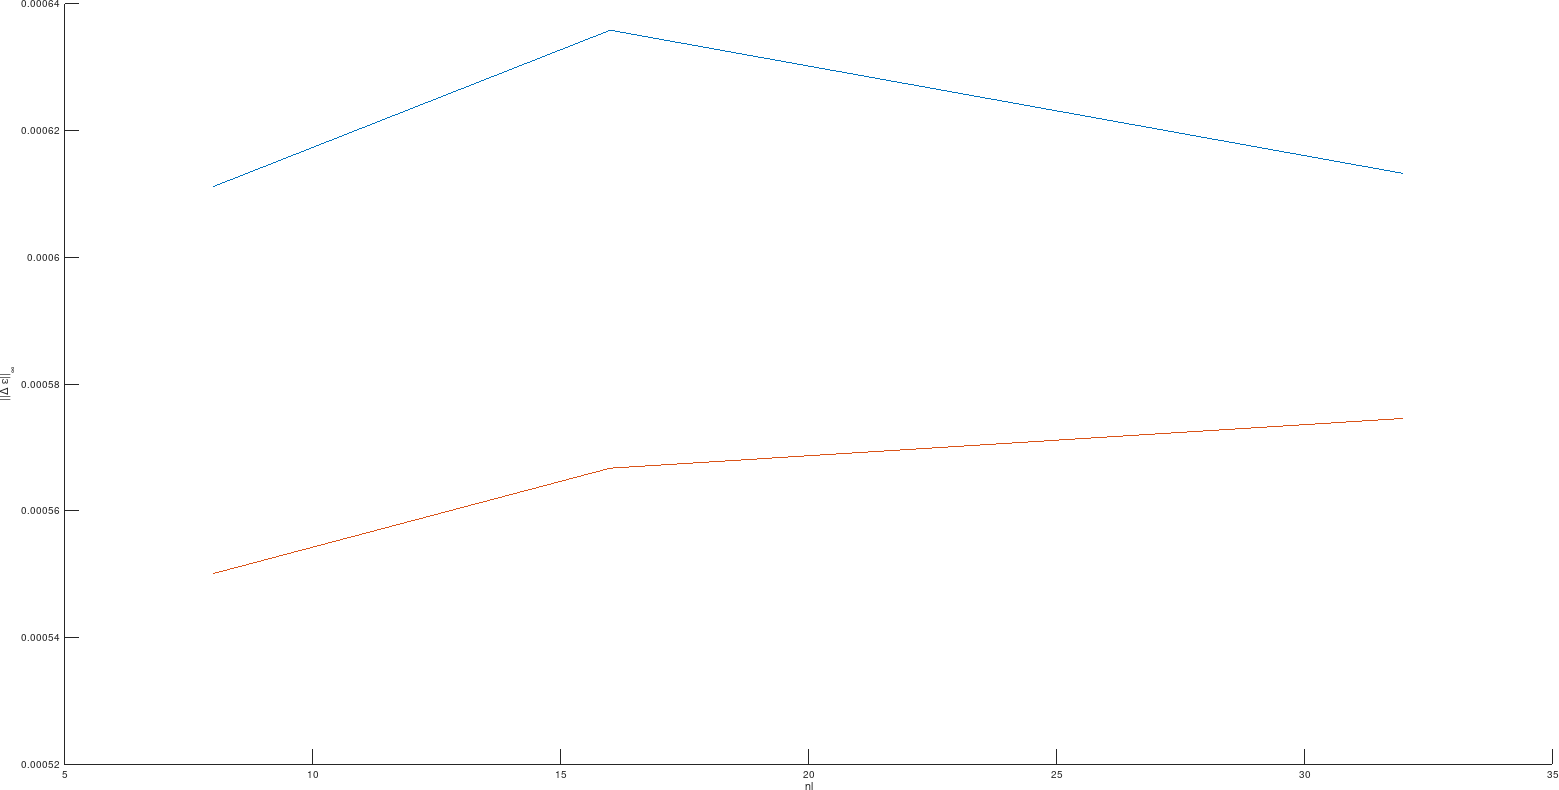
\includegraphics[width=\textwidth]{fig/sc_cvg_rl=4}
   \end{subfigure}
   \begin{subfigure}{0.45\textwidth}
      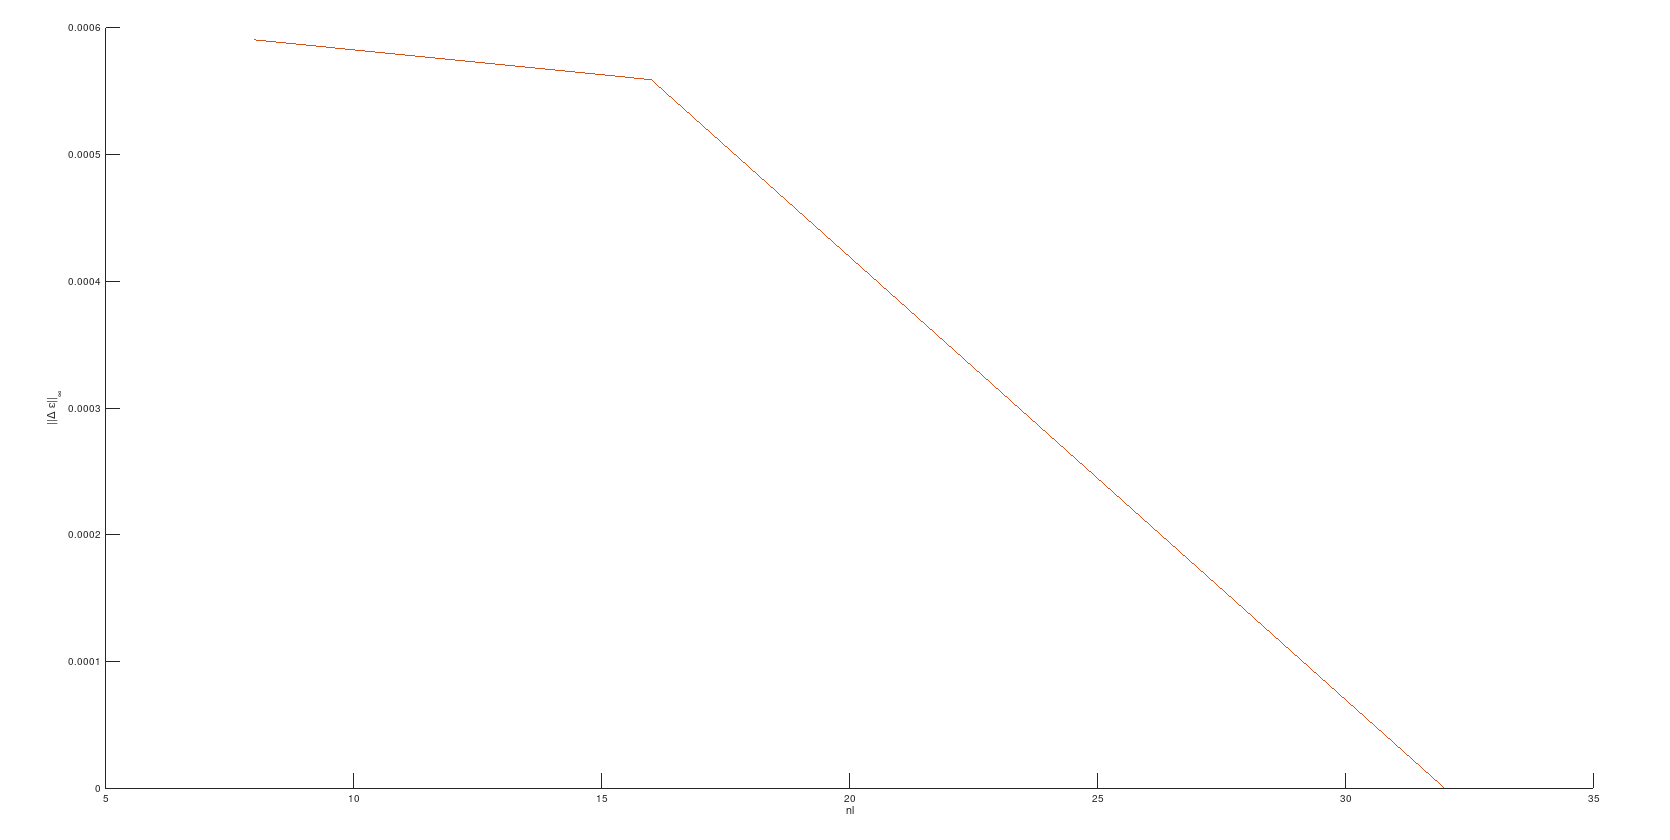
\includegraphics[width=\textwidth]{fig/sc_cvg_rl=5}
   \end{subfigure}
   \caption{normalized transversal emmitance and absolute error of field map in $l_\infty$-norm for $n_I=10$ and $n_l, n_r$ variable}
   \label{fig:sc_cvg_rl}
\end{figure}
\end{center}

\begin{center}
\begin{figure}[H]
   \begin{subfigure}{0.45\textwidth}
      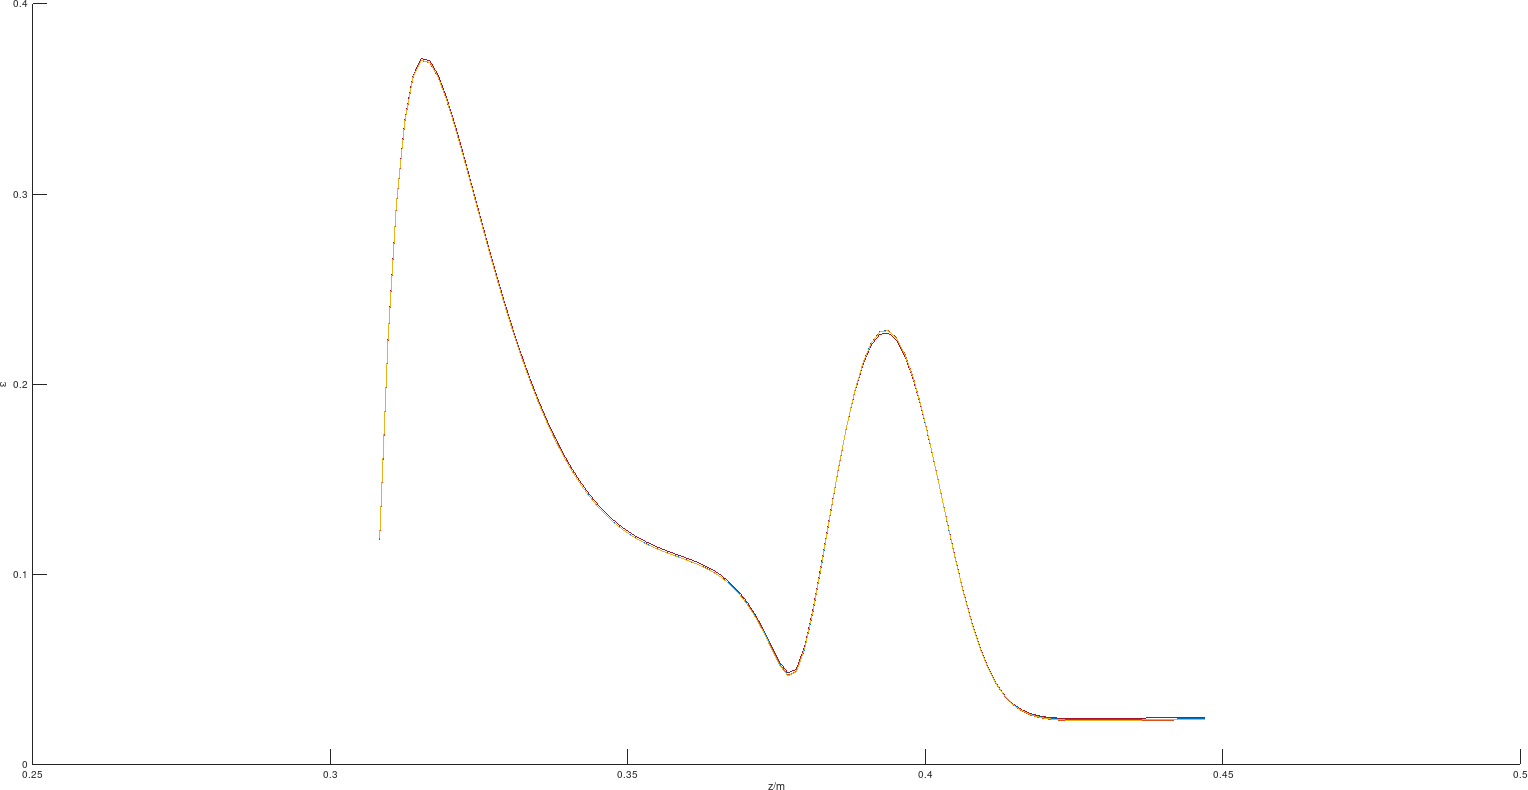
\includegraphics[width=\textwidth]{fig/sc_emit_I}
   \end{subfigure}
   \begin{subfigure}{0.45\textwidth}
      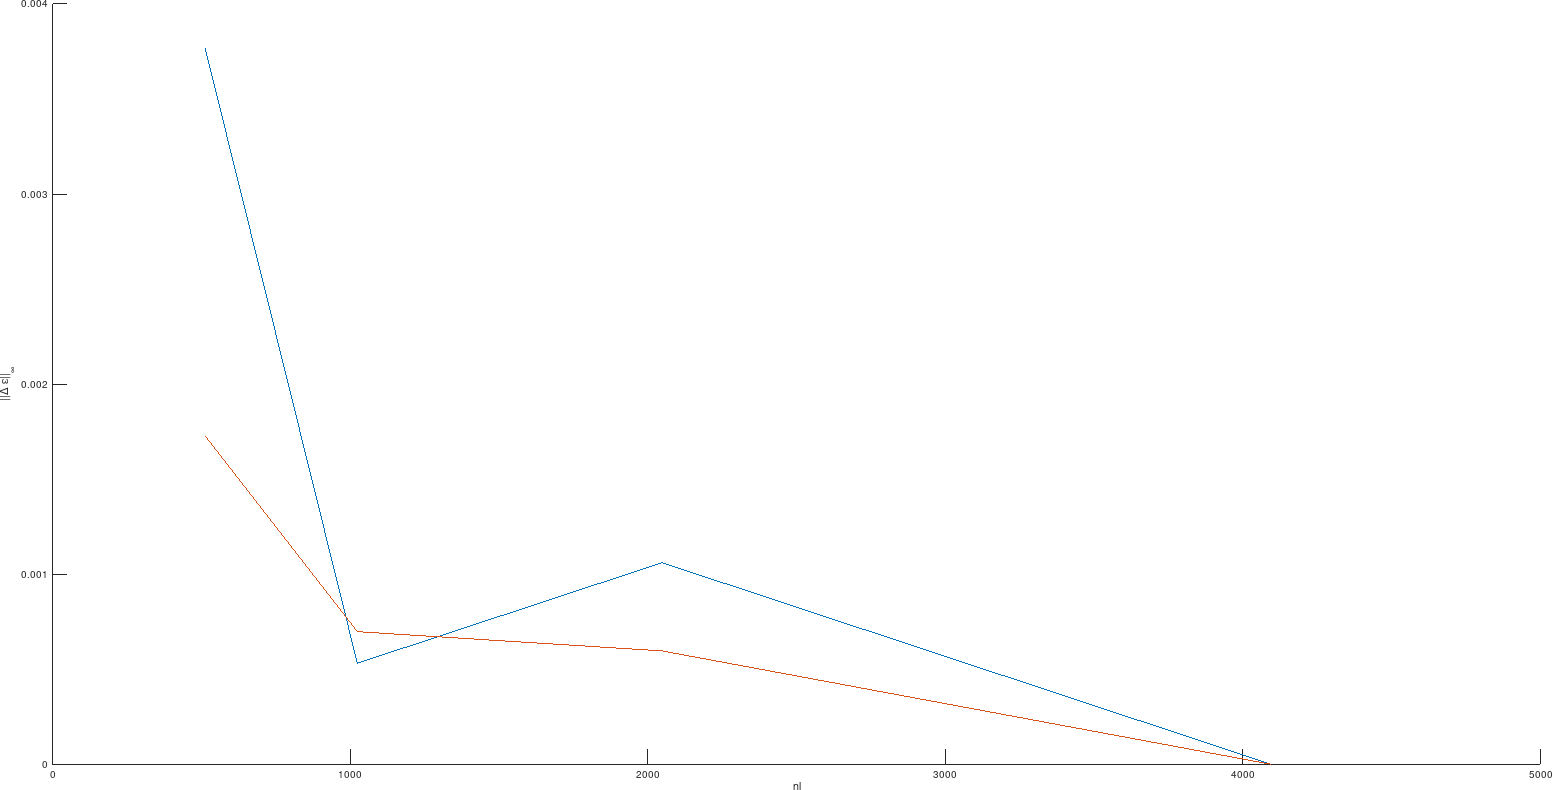
\includegraphics[width=\textwidth]{fig/sc_cvg_I}
   \end{subfigure}
   \caption{normalized transversal emmitance and absolute error of solution in $l_\infty$-norm for $n_I$ variable and $n_l=n_r=4$}
   \label{fig:sc_cvg_I}
\end{figure}
\end{center}

\textbf{TODO}: include plot of initial, optimized tracking and refine plots

\begin{itemize}
   \item \textbf{remarks}: the convergence studies also looked at $x_{rms}$ and the behavior was almost identical to $\epsilon$

   \item to minimize the electric field on the entire electrode surface all curves could be taken into account
   \item also anode ring shape, position and voltage
   \item include tracking to include constraint on $x_\mathrm{rms} \leq 1.5\ \mathrm{mm}$, also optimize or constrain $\epsilon \leq 1\ \mathrm{mrad\ mm}$?
\end{itemize}
